\chapter{State of the art}\label{A:stateOfTheArt}

This chapter aims to provide a vision of how the audio-visual media production sector has been, and still is, carrying out IP convergence. 

Moreover, this chapter will be focused on the topics related to media production over an IP related environment and, specifically, the ones related on this project study and proposal.

\section{IP convergence of media content production}

As briefly as possible, this section aims to summarise the evolution of the IP convergence itself and how technologies are evolving to carry out such transformation at audio-visual media content production level.

Next subsections are also organized by enumerating potential technologies and standards following the OSI \cite{osi} stack from the bottom layer.

\subsection{Physical and Data link layers}

In 1989, SMPTE (The Society of Motion Picture and Television Engineers \cite{smpte}) standardized a family of digital video and audio interfaces based on coaxial cable, called SDI (Serial Digital Interface \cite{SDI}), which is intended to be used for transport of uncompressed digital video and audio in a television studio environment. 

Around SDI there are other related standards which are focused in specific solutions (i.e.: to support higher video resolution, media qualities, media formats, frame rates, audio channels, synchronization,\ldots). An example is the HD-SDI \cite{SDI} standard (High-Definition Serial Digital Interface, defined in SMPTE 292M) which provides bandwidth enough to transport HD video fromats (i.e.: up to 1,485 Gbps). Other SDI related standards are the 3G-SDI \cite{3GSDI} and 12G UHD-SDI \cite{UHDSDI}, which give support to FHD (i.e.: Full HD, 1080p resolution up to 2,970 Gbps bitrates) and 4K (i.e.: UHD cinema resolution up to 12 Gbps bitrates) video formats, respectively. 

Since then, new encapsulation audio (i.e.: AES67-2013 \cite{AES}) and video (i.e.: SMPTE 2022-6 \cite{ST2022}) standards are appearing to transport high-quality media signals over IP Networks.

Also, further specific solutions for manage packet loss recovery using FEC (SMPTE 2022-5) and a seamless protection system (SMPTE 2022-7) have appeared as potential robustness solutions.

In the middle of 2014, the Video Services Forum (VSF) has formed a new group (SVIP) looking at new encapsulation mechanisms for audio, video and ancillary data into IP without using SDI framing (raw data) to develop or recommend a standard for video over IP without SDI encapsulation.

They aim to study and document the requirements for video over IP/Ethernet within plant (i.e.: video, audio, ancillary data, bundles, timing, sequencing, identities and latency) in order to research over current and proposed solutions so that to report on gaps between requirements and existing solutions (especially regarding existing SMPTE 2022 Standards) and finally to propose scope for follow on activity, if required.

Moreover, it is important to remark the Ethernet protocol, which was standardised in 1983 and since then it has been increasing its speed rate from the initial 10 Mbps to 100 Gbps (foreseen 400 Gbps by IEEE P802.3bs Task Force), with currently easily affordable 10 Gbps and 40 Gbps interfaces. These rates seem to be enough to accommodate current broadcast formats (e.g.: HD-SDI at ~1.5 Gbps, 3G-SDI at ~3 Gbps and UHD at ~12 Gbps) and further innovations because of the nature of the packet technologies make them completely agnostic to the upper formats and indeed transparent for future formats in contrast with current media transport technologies which are completely bounded with the transported formats (i.e.: standard cable video formats used over broadcast environments). On another hand, Ethernet hasn't got any timing awareness or QoS assurance, so it makes difficult to accommodate current operation workflows over this technology. Nevertheless, because Ethernet is widely used in the IT industry, its use, as COTS switches, have motivated studies about the use of these switches in the broadcast industry deployments to validate specific necessary features as the latency deviation or packet loss. (REFERENCE: TEST LINK3)

At the same level, to address some of the inherent Ethernet limitations, Audio Video Bridging (AVB) appeared in 2011 which is a set of standard extensions to the Ethernet IEEE 802.1 focusing on timing and QoS guarantee within local area networks. Its approach is a plug-and-play platform to ease transition from current transport technologies to the newer ones using the same workflows, but the current version is still limited to local premises and limited topologies. Since November 2012, because more varied industry sectors joined the task group, a more general name, the Time Sensitive Networking (TSN task group), was created to carry on with the new developments.

On the other hand, the emergence of the SDN paradigm (--REFERENCE--), separating the control and forwarding plane besides creating northbound interfaces to interact with external applications, enables new flexible and customised network operations and deployments. There are a lot of foreseen benefits from this approach but to be fully capable of supporting all type of streams some extensions should appear, such as a specific extension which has been released by the ONF to address timing restrictions known as OpenFlow Time Extension to OpenFlow 1.3.x ext340 (--REFERENCE--).



Related to above statements, the recent advances in chip designs by industry leaders (e.g.: Intel, Broadcom, Xilinx and Altera) have eased a strong movement towards consolidation of complex functions (e.g.: encoding, transcoding, conversion, \ldots ) into a single device, instead
several disparate platforms. Additionally, these hardware advances implied the chance of using software-centric frameworks, which provide for greater flexibility and customization from a business standpoint. Both advances are enabling a broader adoption of upcoming media technologies, at a reduced cost, without compromise on quality, flexibility and capability. Moreover, the disruptive nature of such advances can be seen in the mobile telephony market, such as the entry of open source mobile phone software (e.g.: Google’s Android OS) which, when coupled with low cost but powerful chipsets, has democratised the market allowing millions of people access to mobile phones and with it the Internet.

In parallel, regarding the specific timing and synchronising requirements of live media production, the standard IEEE 1588-2008 (--REFERENCE--), commonly known as PTPv2(--REFERENCE--), appeared covering several profiles to be used through several network environments. For instance, SMPTE(--REFERENCE--) published a draft profile SMPTE ST 2059 (1 and 2) (--REFERENCE--) defining a reference alignment to SMPTE epoch and there are studies analysing the application of PTP to broadcast environments under different circumstances (check this demo LINK4 --> Check also APPENDIX with ieee presentation!).

\subsection{Network and Transport layers}

On the network layer, IP is the de facto standard and within its protocol suite there are some solutions which help to transport media content efficiently. For instance, IP supports multicast paradigm operation using widely supported routing protocols (--REFERENCE--) (e.g.: DVMRP, PIM, IGMP, \ldots), but the computational and scalable complexity of these protocols tends to difficult and limit deployments.

In terms of QoS, IP has a field known as ToS/DSCP (--REFERENCE--) which marks the header packets along their way to help mappings with lower-layer protocols (e.g.: Ethernet or MPLS) to implement QoS at the buffer level.

On the transport layer, UDP has been preferred over TCP for real-time transport because of its connectionless nature and avoidance of unnecessary retransmission for live streams. As common known and basic extension, the RTP (Real Time Protocol), whose most deployed version is RFC 3550, was initially introduced to audio and video services, to add supplementary data fiels in order to enhance the UDP protocol (i.e.: timestamp field, sequence number, payload identification), together with the protocol for control purposes (i.e.: RTCP, which stands for Real Time Control Protocol). Recently, new extensions have appeared introducing new header options to support the adoption of services related to media production workflows. Concretely, RTP and RTCP have been proposed to accommodate media specific info over IP, answering to specific challenges.

\subsection{Application layers}\label{S:sessionPresentationApplicatio}

On another hand, the wide adoption of low-delay encoding (e.g.: JPEG2K, AVC, AVCi, VC-2) for high quality video stream could represent a new opportunity to reduce the bandwidth consumption in several scenarios. Likewise, high-compression mechanism as MPEG4 H264 or HEVC could be
useful to transport media content through very limited network resources scenarios (as Internet or cloud-based systems).

Moreover, specific efforts have risen to arrange specific challenges such as a networked media interface by Sony to carry a virtually lossless UHD/4K (12 Gbps non-compressed) over a single 10 GBE interface or specific implementations facing the switching-point issue. All of these are a useful starting point for future enhancements towards a global operational framework. (RESOURCES/REFERENCES??? LINK5)

Another important issue is the automation of the system to enhance flexibility for deployment set-up and maintenance. Here, some solutions as Zero-configuration networking (-- REFERENCE - LINK6 ) could contribute using well-known protocols as DHCP or DNS-SD to enable auto-configuration and streaming announcement, but to be implemented in an operational scenario a common approach should be defined.

Furthermore, the Telecom Industry introduced the NFV concept (--REFERENCE--) in 2012 to enable the shifting from the hardware-centric approach to the software-centric one. In spite of not being thought for
broadcasting issues, this parading provides new possibilities to bring up new deployments and  enhance current workflows.

In the media plane, protocols as RTSP for end-to-end session control or SDP for service description provide capabilities for the stream management. Furthermore, media wrappers aim to gather different types of programme media and associated information, as well as generically identify this information. Different media wrapper formats are in use at this time (e.g.: MXF --REFERENCE-->>>LINK7), but, for the media industry, it is important that the wrappers have characteristics like openness, extensibility and performance. The MXF (a SMPTE standard) is a “container” format, which supports a number of different streams of coded based by enabling interoperability between different platforms. This is by encoding in any type of video and audio compression formats, together with a metadata wrapper which describes the material contained within the MXF file. Also DDS, a machine-to-machines middleware standard from OMG (--REFERENCE--), could be used to enable interoperable media exchange between actors. At the same time, EBU has launched the FIMS (Framework for Interoperable Media Services --REFERENCE--) which intends to answer to different interoperability issues between SOA proprietary systems by defining an open, consensual framework with standardised interfaces.

Regarding the measurement of media transport over IP, VSF published in 2006 a document (RVOIM LINK8 ) to define the recommended metrics for Video over IP transport. The aim of the document is help in the monitoring, troubleshooting and equipment performance compliance to standards and specifications, verifying and measuring the delivered services statistics and equipment analysis and debug.

As could be inferred from the above statements, there are no current common approach to solve the whole challenge yet. To face this issue some initiatives have appeared lately. Many outstanding research initiatives are on the way but an interesting one was carried out by the BBC (--REFERENCE - LINK9) which tried to provide an operational framework for a live studio within their environment.

Likewise, in 2013 SMPTE, VSF and EBU created the JT-NM task force (JTNM) to drive the broadcasting industry towards a full IP adoption by providing guidelines to enable a successful migration. Currently, the JT-NM is working to develop a reference architecture to help all involved layers to agree on all cross issues whereas defining specific requirements over concrete use cases to uncover missing definitions to address the general scenario (--REFERENCE -- LINK10).

\section{Migration to cloud}

This section is a continuation of the previous one but focusing on how OTT content technologies are giving new chances to enhance audio-visual media production to IP convergence, concretely within the cloud computing concept. 

\subsection{Cloud computing}

Cloud computing describes the delivery of shared computing resources (software and/or data) on demand through the Internet and its benefits can be foreseen as it is defined by the NIST recommendations (--SEE APPENDIX X OR REFERENCE--). So, for many reasons like flexibility, scalability, security, data protection, agility and cost many organisations are migrating to cloud computing environments. 

Nowadays, cloud computing defines three fundamental models that are organized through application/service, platform and infrastructure layers.

\begin{figure}[htb]
\begin{center}
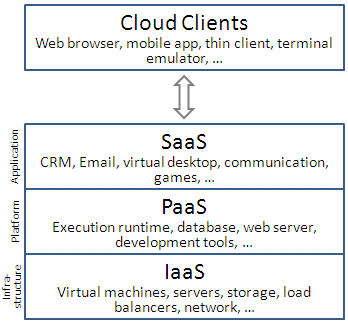
\includegraphics[width=0.6\textwidth]{./images/Cloud_computing_layers.png}
\caption{Cloud computing layers}
\label{F:cloudComputingLayers}
\end{center}
\end{figure}

Moreover, there are different deployment models depending on the product behind (e.g.: specific service or application), which are the resources from the entity that is offering or using such product. Main deployment models might be:

\begin{itemize}
\item Public: when applications/services run over a network that is open for public use, which may be free. The fact of being public/opened implies much more complexity in terms of security issues.
\item Private: when infrastructure is operated solely for a single organization, whether managed internally or by a third-party, and hosted either internally or externally. This cloud type might be similar in terms of architecture design from the public one.
\item Hybrid: when a composition of two or more clouds (private or public ones) are treated as distinct entities but are bound together, offering the benefits of multiple deployment models. Hybrid cloud allows to extend the capabilities of a cloud service by aggregation, integration or customization with another cloud service.
\end{itemize}

To point out that high-performance computing (e.g.: GPU based clouds --REFERENCE--) and software-defined networking (SDN) could improve solutions to current cloud issues such as security, processing performance, full processing chain control through specific SLAs, among others.

So, in many terms, the cloud concept is a key solution to help media producers create better content more quickly and there are lots of examples to focus on, but lets introduce the ones that tends to flexible and scalable ways to access the benefits that cloud computing brings to media production:

\begin{itemize}
\item Low-cost initial expenditures \hfill 

Media production tends to require an enormous initial investment in technology infrastructure and the technical staff to manage it. In that sense, cloud computing technology is that the creative industries are alleviated of the need to invest heavily in technology that would rapidly become obsolete. Cloud computing allows the media production industry to provision only the technology they need, when they need it, avoiding excessive CAPEX.

\item Cost forecasting\hfill 

Infrastructure as a Service (Iaas) prices are predictable and granularly treated. It allows prediction on a per project basis with detailed cost analysis precision. As done by many IaaS providers (e.g.: Amazon and Woowza), each resource used in a media production workflow is metered, and companies pay only for what they use.

\item Dynamic infrastructure deployment \hfill 

Cloud computing helps production entities take advantage by the on demand basis applied deployments. Media production companies can quickly provision servers to meet the demands of specific projects and shut them down when they are no longer needed.
\end{itemize}

Moreover, cloud computing can improve media production at many different media services requirements planes, such as:

\begin{itemize}
\item Media asset management
\item Granular costs measurement
\item Cloud transcoding
\item High-speed file transfer
\item Automated content verification
\item Elastic deployment
\item Real-time and full monitoring
\item Video quality control
\end{itemize}

And, expected overall outcomes might be:

\begin{itemize}
\item Increased performance
\item Lowered costs
\item Improved cross collaboration
\end{itemize}

As a subchapter corollary, figure \ref{F:cloudComputingLayers} describes generic cloud computing layers, but it also refers to this project's topics in order. These are virtualization, monitoring concepts and the service that is going to be deployed and tested which is implemented using the LiveMediaStreamer framework.

\subsection{Virtualization}\label{SOA:Virtualization}

Cloud computing is usually strongly related and implemented with different kinds of virtualization. Many virtualization methods are commonly implemented at datacenters where platforms and services are going to be deployed over different infrastructure architectures. Nevertheless, deploying virtualization at data centers doesn’t automatically mean running over a cloud and it’s possible to deploy clouds without virtualization. Furthermore, as well as cloud computing concept started to be widely used from 2000's, virtualization  technologies can be traced back to the 1960’s such as virtual desktops, but others can only be traced back a few years, such as virtualized applications (--REFERENCE-- LINK11).

Specifically, virtualization under computing environments means creating a virtual version of any possible piece of actual hardware or software so that we can use system resources effectively. Despite of many ways to define current virtualization methods, the following statement is proposed and it's defined by types and levels:

\begin{itemize}
\item Types: based on specific computer/server resources virtualization. These are: 
\begin{itemize}
\item Data virtualization: when an application is able to retrieve and manipulate data without requiring technical details of such data.
\item Memory virtualization: when, in a cluster, volatile random access memory (i.e.: RAM) resources are decoupled from physical machines in order to be aggregated with other RAM resources and to become a virtualized memory pool.
\item Network virtualization: when combining hardware and software network resources and network functionalities into a single and software-based management entity.
\item Storage virtualization: when pooling data from multiple and different storage devices into a virtual device that is managed from a central console.
\end{itemize}
\item Levels: based on abstract and generic virtualization concepts. These are:
\begin{itemize}
\item Application virtualization: when encapsulating an application software from the underlying operating system on which it is executed. It involves separating the physical client device from the management of the application itself.
\item Environment virtualization: when virtualizing at operating system level. It's a virtualization method where the kernel of an operating system allows for multiple isolated user-space instances, instead of just one. 
\item Hardware virtualization: when hiding the physical characteristics of a computing platform from a user point of view and showing another abstract computing platform. It means computer or operating system virtualization by creating virtual machines.  Nowadays, the software that manages virtualization is called hypervisor or virtual machine monitor.
\end{itemize}
\end{itemize}

Therefore, in terms of cloud computing benefits, virtualization can increase agility, flexibility, and scalability while creating significant cost savings. Workloads might be deployed faster, performance and availability increases and operations can become fully automated, resulting in a cloud with ease to be managed. 

Although the virtualization types that are defined, this subchapter is focusing on the previous defined virtualization layers, which are of interest for this project development.

So, starting from the upper layer, application virtualization's current technologies are (--REFERENCE--):

\begin{itemize}
\item Desktop virtualization: when separating part or all of the desktop environment and associated applications from the physical client device that is used to access remotelly or locally it. This improves portability, manageability and compatibility of a personal computer's desktop environment. A common implementation of this approach is to host multiple desktop operating system instances on a server hardware platform running a hypervisor. This is generally referred to as Virtual Desktop Infrastructure (i.e.: VDI). Some commercial examples are RemoteApp of Microsoft and the Seamless Windows of Citrix. 
\item Application streaming: when delivering pieces of the application's code, data, and settings when they're first needed, instead of the entire application being delivered before startup. Running the packaged application may require the installation of a lightweight client application. Packages are usually delivered over a protocol such as HTTP, CIFS or RTSP. Some examples are Microsoft App-V and Citrix XenApp Streaming.
\end{itemize}

Next layer is the intermediate layer of environment virtulization. Pioneer implementation was FreeBSD jails mechanism allowing system administrators to partition a FreeBSD-based computer system into several independent mini-systems called jails. There are many other examples of environment virtualization, but all of them are OS-based virtualization with differences like its kernel operating system (i.e.: FreeBSD, Solaris, Unix-like, and Windows) and the level of isolation in terms of resources utilization (i.e.: types of virtualization, above explained), security and ease of delegation. 

Currently, the environment virtualization method of Linux containers (LXCs) are widely enhancing application/services development, testing, packaging, deployment and managing methodologies. Specifically, containers represent one of the leading trends in computing today. With companies such as Docker, CoreOS, ClusterHQ joining industry giants like IBM, Red Hat, MIcrosoft and others. A recent study by DevOps.com and ClusterHQ showed that over 90\% of organizations have either looked at or plan to look at containers in the near future (--REFERENCE--).

Finally, the lower environment virtualization layer is the hardware-centric one. Different methods can be distinguished as follows:

\begin{itemize}
\item Full virtualization: when simulating enough hardware to allow using an isolated guest operating system in a virtual machine. There are many examples of implementation like Parallels, VirtualBox, OracleVM, VMware and QEMU among other platforms.
\item Hardware-assisted virtualization: is a full virtualization enhancement that uses specific hardware capabilities by improving hardware simulation efficiency. There many implementations' examples like Linux KVM and Xen among others platforms. 
\item Partial virtualization: was the previous virtualization technology of the full virtualization. Main differences resides on the address space virtualization, in which each virtual machine consists of an independent address space. This fact implies that a full operating system is not able to run in a virtual machine but many of its applications. 
\item Paravirtualization: when a virtual machine does not implement full hardware virtualization, but offers a special API for a guest with a modified version of the operating system. This type of virtualization is also implemented in most of the widely used virtualization platforms like VMware, Parallels and Xen.
\end{itemize}

\subsection{Monitoring}\label{SOA:monitoring}

Strongly related to cloud reliability is the monitoring concept. In order to reach maximum cloud reliability it's important to observe and check the progress and/or quality of key parameters over certain periods of time and to keep them under systematic review in order to create proper reactions, if required.

Therefore, this implies monitoring the cloud infrastructure (e.g.: servers, virtual or physical) and related services (e.g.: applications). Here appears the QoS (Quality of Service) and QoE (Quality of Experience) terms, respectively.

QoS is the network-centric monitoring of underlying infrastructure components such as servers, routers and its network traffic. QoS metrics are generally device (e.g.: CPU and memory load, CPU temperature, disk space or HDD health) or transport-oriented (e.g.: packet loss, delay, bandwidth usage or jitter). 

Although QoS can be fully affordable due to the robustness and redundancy of current infrastructures (e.g.: back-up services, network rerouting and error correction), this doesn't mean that any end user might be feeling comfortable by using deployed services (e.g.: searching on a e-commerce webpage) over a high QoS infrastructure. Then, QoE monitoring term evaluates the quality delivered to a user and it's done by analysing parameters when connecting to such services like a user. Therefore, QoE performance indicators are user-centric (e.g.: webpages response time or measuring video and audio quality (MOS)).

Common network monitoring protocols for distributed infrastructures management are:

\begin{itemize}
\item SNMP: Simple Network Management Protocol is a widely known and used Internet standard protocol for managing IP-capable devices (i.e.: devices that implements SNMP)
\item WMI: Windows Management Instrumentations is a Microsoft's implementation of the Web-Based Enterprise Management (WBEM) and Common Information Model (CIM) standards from the Distributed Management Task Force (DMTF).
\item NetFlow: a Cisco protocol for network switches and routers.
\end{itemize}  

Usually, these protocols are used to measure QoS, but there are complex algorithms that processes those QoS measurements parameters of interest in order to measure the QoE too. Nevertheless, there are specific applications to define and perform specific QoE measurements. These are known as bots or robots.

Going to what this project is about, the QoE measurements are relevant for audiovisual content services because bad network performance may highly affect the user's experience. This is mainly because these contents are compressed and coded, and have low entropy. Moreover, when designing systems, for referenced analysis, several elements in the video production and delivery chain may introduce distortion by degrading the content (i.e.: from the transcoding system, transport network, access network, home network to end device).

On the other hand, the referenceless analysis is based on the idea that end users don't know about the original content. In this case, instead of measuring the QoE by comparing the original data to the delivered one, this is done by trying to detect artefacts (i.e.: blockiness, blur or jerkiness for video frames).

Typically, the evaluation of the QoE for audiovisual content provides users with a range of potential choices (i.e.: low, medium and high quality levels) that are currently widely accepted.

Obviously, the automation of critical cloud performance monitoring tasks is crucial for ensuring availability, providing efficient services and reducing common errors, costs and complexity. So, the use of OTT applications that processes such quantities of data flows and displays outcome parameters of interest are crucial. 

There are many tools that offer monitoring capabilities to be integrated and of-the-shelf. Such monitoring capabilities can be organized as:

\begin{itemize}
\item System monitoring \hfill

Single server/computer/instance resources monitoring (e.g.: CPU and memory loads or processes utilization). Typical examples are the system monitoring tools that each operating system comes with by default.
\item Network monitoring \hfill

Related to previous item, but specific to network resources monitoring (e.g.: monitoring input and output accumulated bytes of a single computer network interface or monitoring specific network hardware like accumulated incoming UDP packets of a router in a LAN). Most of related tools are based on network monitoring protocols implementations in order to perform as a distributed monitoring unit. But, there are many examples of tools and services for network monitoring which goes from desktop applications (e.g.: netstat or iptraf) to specific router and switch daemons (e.g.: MRTG).
\item Infrastructure monitoring \hfill

When coupled system and network monitoring together by adding specific tools and interfaces to monitor distributed resources within the infrastructure. There are many examples of tools  (e.g.: cactix or monitis) and services (e.g.: new relic or pingdom) at this monitoring level.
\end{itemize}

The associated database model for collecting such amount of data is the widely known Round Robin Database, which stores data in a circular buffer based database where the system storage remains fixed by handling time-series data. 

Finally, to remark that network managers have the capability to minimize the storage and network resources by allocating only the resources that are required thanks to monitoring evaluation services and tools.

\subsection{Application}\label{SOA:coreService}

This subsection aims to remark the importance of designing and deploy a well structured application/service architecture over the cloud. Therefore, it's important to showcase most common and current application architecture patterns before designing a proper platform prototype.

\subsubsection{Services based architectures}\label{SOA:appArch}

There are two main architecture patterns of interest for services architecture definitions over networks. 

\begin{itemize}
\item Service Oriented Architecture (SOA) \hfill

SOA is software architecture pattern where application components provide services between other components (services) through different types of communications protocols. Services can be combined to provide the functionality of a full software application.
This pattern defines the services as logical representations of a repeatable business activity with specific goals (i.e.: statistics monitoring)

\item Microservices architecture \hfill

Microservices is a software architecture pattern in which complex applications are composed of small, independent processes communicating with each (microservices) other using language-agnostic APIs. These services are small, highly decoupled and focus on doing a small task, facilitating a modular approach to system-building. 
Microservices is rather different than SOA perspective: microservices are always independently deployable in their own processes  (-- REFERENCE FORVES--)

\end{itemize}

Without going too deeply on both architecture patterns (check out its references --APPENDIXES--), it seems that for this project requirements a microservices pattern offers more flexibility and lets define a proper architecture where services can be or can't be splitted (i.e.: modules of the same binary process or communication protocols improvements with APIs) when required. 

The prototype to be proposed should be seen as a complex application (the production platform) that requires defining specific microservices that can run independently and require to be flexible in terms of creating different interconnections per each possible configuration.
 
\section{LiveMediaStreamer}\label{SOA:LMS}

This section is devoted to the framework which the core service (i.e.: audio and video mixer software) to be analysed is implemented with, the LiveMediaStreamer (LMS) framework. 

\subsection{LMS framework}\label{SOA:LMSframework}

LMS framework has been developed with my team work since two years ago. A first implementation was based on the network core of the open-source software UltraGrid (--REFERENCE--). One year after, a new core has been developed based on the network streaming library Live555. This change has improved system performance and ease further developments. Live555 library enables implementing any RTP and RTSP module, standard or not, among offering out of the box specific audio and video RTP payload formats support like H264, HEVC or VP9 for video codecs and G711, OPUS or AAC for audio codecs.

The aim of LiveMediaStreamer framework is to offer multiple audio and video streams manipulation in real-time in many ways. It is designed following a pipeline pattern so that it consists in a number of filters (i.e.: encoders, decoders, receivers, transmitters, dashers, mixers and resamplers) that can be concatenated or connected with each other in order to process a data flow. The framework is developed under a Linux environment, currently being the only supported platform, using C++ standard libraries and it makes use of several mature media related libraries, which are: 

---REFERENCES FOR EACH ONE---
\begin{itemize}
\item Live555 – Network streaming media library which implements the RTP standard protocol.
\item ffmpeg – A complete, cross-platform solution to record, convert and stream audio and video.
\item OpenCV – Open source computer vision and machine learning software library.
\item x264 – Free software library and application for encoding video streams into the H.264/MPEG-4 AVC compression format.
\item x265 HEVC Encoder – Open source HEVC encoder.
\item LAME – High quality MPEG Audio Layer III (MP3) encoder licensed under LGPL license.
\item Opus – Totally open, royalty-free, highly versatile audio codec.
\item WebM VPX – VP8/VP9 Codec SDK. A open, royalty-free, media file format designed for the web.
\end{itemize}
 
The framework is designed to be managed remotely through a simple network interface based on JSON formatted TCP socket messages. 

Currently, the framework does not have a RESTful API, but has a web API based middleware, that loads and manages an audio and video mixer scenario, written in Ruby programming language and it implements Sinatra framework for the web service interface side.

It's recommended to check APPENDIX \ref{ANX:lmsarchfull} for more information about specifics of the LMS architecture in order to understand next chapters (mostly, in problem statement and proposal's subchapter \ref{B:appLayerCH2} and chapter \ref{D:application}, the solution's implementation).

\subsection{Existing similar solutions}\label{SOA:similarSolutions}

Finally, it is important to showcase the current state of the art regarding similar technologies.

Most notable audio and video production-like technologies over networks are:

\begin{itemize}
\item Wowza \hfill
 

\item Red5 \hfill


\item Adobe Flash Media Server \hfill


\item vMix \hfill


\item makeTV \hfill


\item Telestream Wirecast \hfill


\item Anvato \hfill


\item Livestream \hfill

\end{itemize}

There are other technology/application combinations that lend to deploy a media production platform.

POTSER FER UNA TAULA

\begin{table}[htb]
\caption{Exemple de taula}
\begin{center}
\begin{tabular}{|c|l|r|}
\hline
{\bf Títol de la Columna 1} & {\bf Títol de la Columna 2} & {\bf Títol de la Columna 3}  \\ \hline \hline
centrada        & a l'esquerra    & a la dreta       \\ \hline
centrada        & a l'esquerra    & a la dreta       \\ \hline
centrada        & a l'esquerra    & a la dreta       \\ \hline
centrada        & a l'esquerra    & a la dreta       \\ \hline
centrada        & a l'esquerra    & a la dreta       \\ \hline
\end{tabular}
\label{T:prova}
\end{center}
\end{table}
